\documentclass[10pt,english]{beamer}
%\documentclass[english,handout]{beamer} % For handouts
\input{../metropolis_preamble.tex}
\input{../macros.tex}
%\usepackage{extendedalt}
%\usepackage{animate} % Animations
%\usepackage{../lindsten}
%\usepackage{movie15}
\usepackage{tikz}
\usepackage{listofitems} % for \readlist to create arrays
\usepackage{booktabs}

\title{732G57 Maskininlärning för statistiker}
\subtitle{Föreläsning 4}
\date{}
\author{Josef Wilzén \\ IDA, Linköping University, Sweden}
\titlegraphic{\hfill
\includegraphics[height=1.2cm]{../LiU_primary_black.pdf}}
%\institute{Joint work with\dots}


%% MY DEF %%
\newcommand{\itm}[1]{\mathrm{Item}_{#1}}
\newcommand{\pausa}{\pause}
%\renewcommand{\pausa}{}
\tikzstyle{mynode}=[thick,draw=blue,fill=blue!20,circle,minimum size=22]

\hypersetup{
  colorlinks=true, urlcolor=blue, linkcolor=red
}

\newenvironment{nscenter}
 {\parskip=0pt\par\nopagebreak\centering}
 {\par\noindent\ignorespacesafterend}

\begin{document}

\maketitle

\begin{frame}{Dagens föreläsning}

    \begin{itemize}
        \item K-närmaste grannar
        \item One-Dimensional Kernel Smoothers
        \item Lokal Regression
        \item GAM: Generaliserade Additativa Modeller
    \end{itemize}
    
\end{frame}

\begin{frame}{K-närmaste grannar}
    \begin{greenbox}
        \myheading{Idé} basera predikation på de K datapunkter som är närmast.
   \end{greenbox}

   Ger en icke-parametrisk metod för klassificering och regression.

   Problem: Vad är närmast?
\end{frame}

\begin{frame}{Avståndsmått}
    Vi behöver något som talar om för oss hur nära två datapunkter är. Finns många alternativ som man kan välja, som ger olika resultat.

    \begin{description}
        \item[Euklidiskt avstånd]
        \begin{equation*}
            d(\mathbf{x},\mathbf{y}) = \sqrt{\sum_{k=1}^{p} (x_k - y_k)^2}
        \end{equation*}
        \item[Manhattan avstånd] 
        \begin{equation*}
            d(\mathbf{x},\mathbf{y}) = \sum_{k=1}^{p} | x_k - y_k |
        \end{equation*}
    \end{description}
\end{frame}

\begin{frame}{K-närmaste grannar - klassificering}
    \begin{enumerate}
        \item Låt $k$ vara ditt valda antal grannar och $D$ din träninigsdata.
        \item För varje testdata $z = (\mathbf{x}', y') \in D$:
        \begin{enumerate}
            \item Beräkna $d(\mathbf{x},\mathbf{x}')$ (avstådet mellan $z$ och all träningsdata)
            \item Välj $D_z \subseteq D$, de $k$ närmaste träniningsdatan till $z$
            \item Låt $y' = \argmax_v \sum_{(\mathbf{x}_i, y_i) \in D_z} \mathbf{I}_{v = y_i}$
        \end{enumerate}
    \end{enumerate}
    2.3 är majoritetsval. Kan också vikta detta värde med avståndet:
    \begin{itemize}
        \item[2.3] $y' = \argmax_{v} \sum_{(\mathbf{x}_i, y_i) \in D_z} w_i \mathbf{I}_{v = y_i}$. 
    \end{itemize}

    För regression används medelvärde, alternativt viktat medelvärde.
\end{frame}

\begin{frame}{K-närmaste grannar}

    %
\includegraphics[]{figs/kernel.png}
    
\includegraphics[scale=0.3]{/home/joswi05/Dropbox/Josef/arbete/kurser/732G12/732G12_2024HT/732G12_DM/lectures/lecture4/fig/KNN_fit_data.png}
    
\end{frame}


\begin{frame}{K-närmaste grannar}

    \begin{itemize}
        \item Målet med modellen är att prediktera nya observationer 
        \begin{itemize}
          \item $\rightarrow$ enkel/lat metod
        \end{itemize}
        \item Avståndsmått påverkar, påverkas stort av olika skalor på variabler
        \item Långsam anpassning.
        \item Känslig mot brus.
        \item Val av K har stor betydelse!
        \begin{itemize}
            \item Litet K ger överanpassning.
            \item Stort K ger underanpassning.
            \item Korsvalidering kan användas för att bestämma K.
        \end{itemize}
        \item Producerar godtyckligt utformade beslutsgränser.
        \item Problem i högre dimensioner $\rightarrow$ \href{https://en.wikipedia.org/wiki/Curse_of_dimensionality}{ Curse of dimensionality}
       
    \end{itemize}
    
\end{frame}


\begin{frame}{K-närmaste grannar: exempel}

    Regressionsdata: röda linjen + brus
    \begin{equation*}
        \hat{g}(x) = \operatorname{Medel}(y_i | x_i \in N_k(x)).
    \end{equation*}

    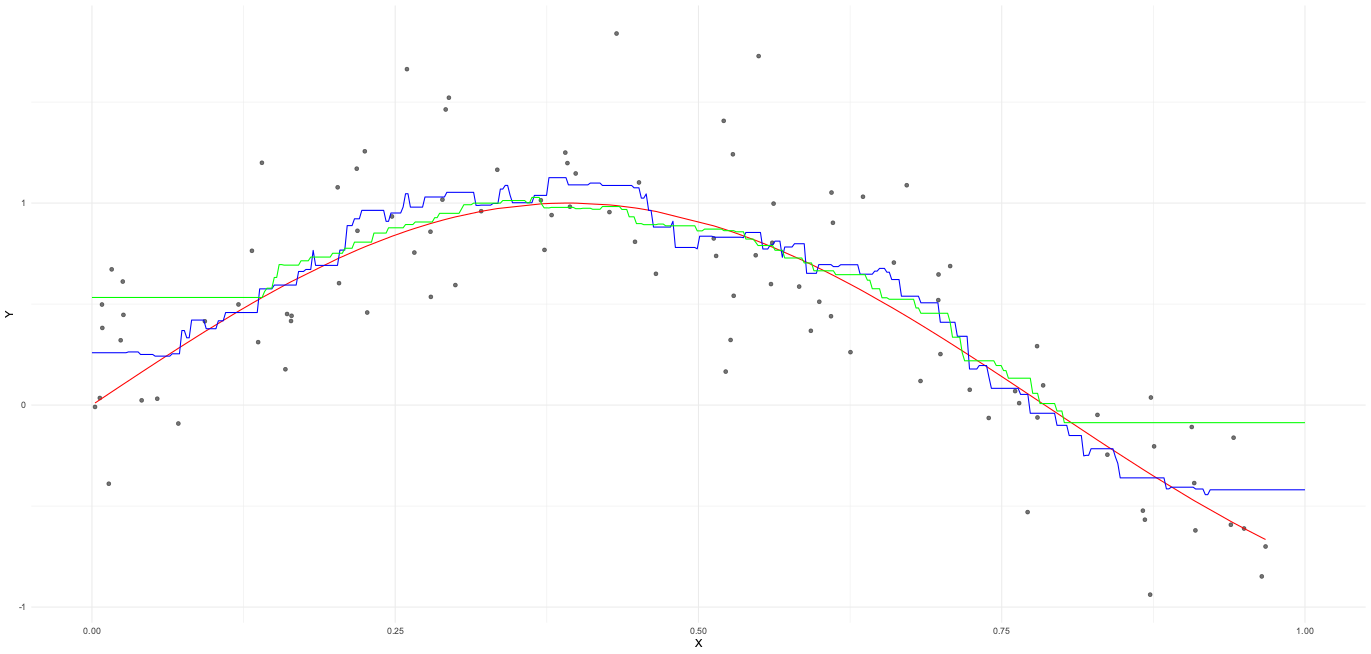
\includegraphics[width=\textwidth]{fig/knnreg.png}

    KNN: Blå har $K=10$ och grön har $K=30$.
\end{frame}



\begin{frame}{One-Dimensional Kernel Smoothers}

    \begin{itemize}
        \item KNN-regression ger samma vikt till alla punkter i grannskapet.
        \item Detta kan ge hopp och en ojämn skattad funktion.
        \item En lösning är att låta vikten bero på avståndet till $x_0$.
    \end{itemize}

    \medskip

    Vi vill skatta $g(x_0)$ och använder ett viktat medelvärde:

    \[
        \hat g(x_0)
        =
        \frac{
            \sum_{i=1}^{n}
            K_{\lambda}(x_0,x_i)y_i
        }{
            \sum_{i=1}^{n}
            K_{\lambda}(x_0,x_i)
        }.
    \]

    \medskip

    \begin{itemize}
        \item Observationer nära $x_0$ får hög vikt.
        \item Observationer långt från $x_0$ får låg vikt.
        \item $K_{\lambda}(x_0,x_i)$ kallas en \emph{kernel} eller viktfunktion.
    \end{itemize}

\end{frame}


\begin{frame}{One-Dimensional Kernel Smoothers}

    En kernel används för att ge större vikt till punkter nära
    \(x_0\) och mindre vikt till punkter längre bort.

    \[
        \hat g(x_0)
        =
        \frac{\sum_{i=1}^n K_\lambda(x_0,x_i)\,y_i}
             {\sum_{i=1}^n K_\lambda(x_0,x_i)}
    \]

    \vspace{0.3cm}

    Vanliga kernels:

    \begin{itemize}
        \item Triangel
        \item Epanechnikov
        \item Quartic
        \item Gaussian
    \end{itemize}



\end{frame}


\begin{frame}{One-Dimensional Kernel Smoothers}

    \begin{block}{Bandwidth}
        Hyperparametern \(\lambda\) styr hur stort område kring
        \(x_0\) som påverkar skattningen.
    \end{block}

    \begin{itemize}
        \item Litet \(\lambda\) $\rightarrow$ låg bias, hög varians.
        \item Stort \(\lambda\) $\rightarrow$ hög bias, låg varians.
        \item Valet av \(\lambda\) är ofta viktigare än valet av kernel.
    \end{itemize}

\end{frame}


\begin{frame}{One-Dimensional Kernel Smoothers}

    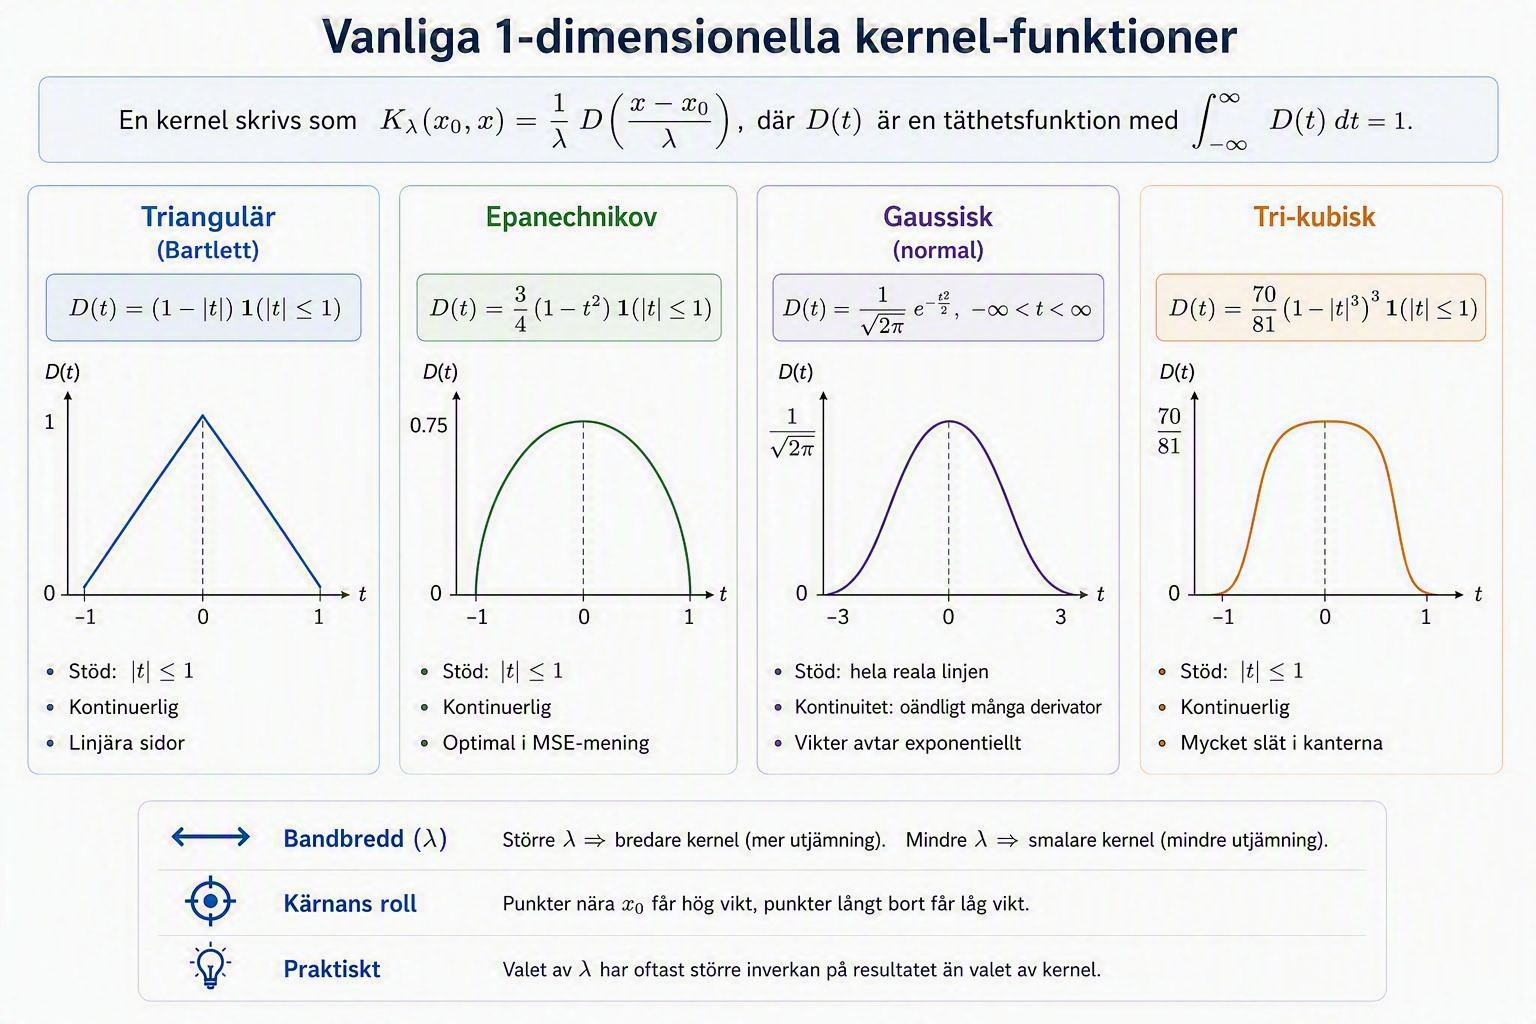
\includegraphics[width = \textwidth]{fig/kernel_plot3.png}
    
\end{frame}



\begin{frame}{One-Dimensional Kernel Smoothers}

    Vi testar tre olika kernels (Triangel - Grön, Epanechnikov - Brun, Quartic - Blå) och får följande resultat

    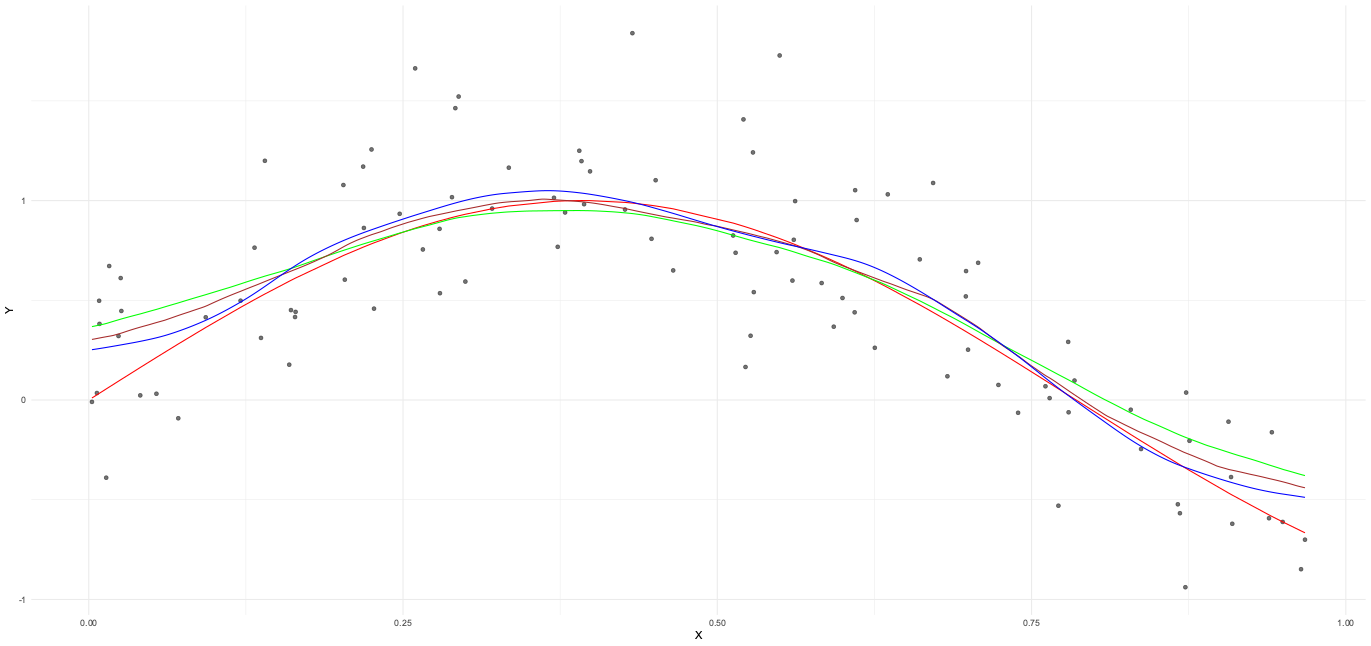
\includegraphics[width = \textwidth]{fig/kernel.png}
    
\end{frame}

\begin{frame}{One-Dimensional Kernel Smoothers}

    \begin{itemize}
        \item Ett sätt att göra "viktat KNN" som ger en "mjuk" funktion.
        \item Vanligtvis sätter vi inte ett antal grannar.
        \begin{itemize}
            \item Låter $\lambda$ styra hur stort fönster vi kollar i.
        \end{itemize}
        \item Många olika val av kernels.
        \item Valet av \(\lambda\) är ofta viktigare än valet av kernel.
        \item Problem vid kanterna.
    \end{itemize}
    
\end{frame}

\begin{frame}{Lokal Regression}

    Vi har sedan tidigare delat upp variabelrummet i olika delar och gjort regression på varje del.

    Istället för att dela upp rummet i förväg och göra regression i varje del, varför inte välja ett intervall runt den punkt där vi vill beräkna regressionen?

    Hur välja område?
    
\end{frame}

\begin{frame}{Lokal Regression}
    Inspirerat av det One-Dimensio Kenel Smoothers
    \begin{greenbox}
        Gör (linjär) regression vid en punkt $x_0$ där vi viktar alla fel med en kernel.
    \end{greenbox}

    För varje punkt $x_0$ där vi vill beräkna funktionen löser vi ett regressionsproblem
    \begin{equation*}
        \min_{\mathbf{\beta}(x_0)} \sum_{i=1}^{n} K_{\lambda}(x_0, x_i) [y_i - \beta_0(x_0) + \beta_1(x_0) x_i]^2.
    \end{equation*}

\end{frame}

\begin{frame}{Lokal Regression}
    Skattar lokal regression med olika $\lambda$ och Tri-Cube

    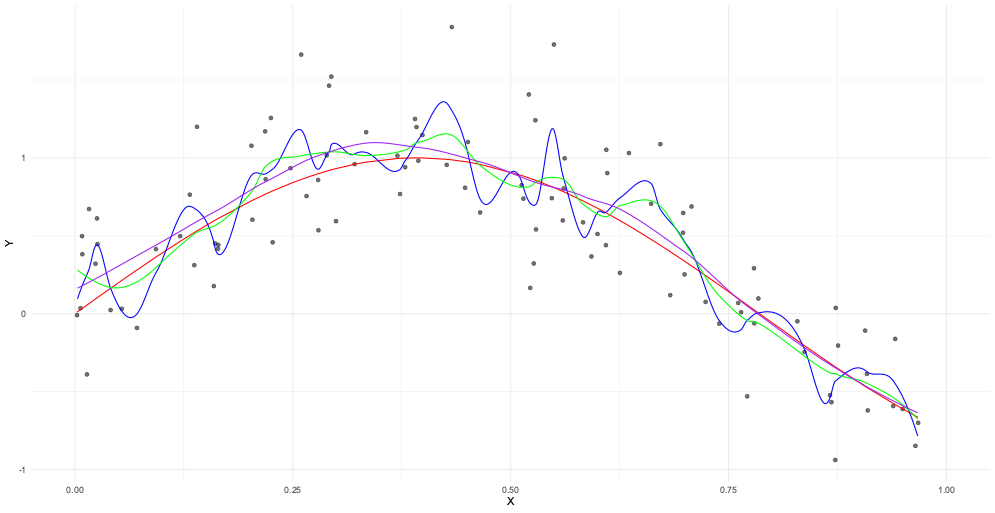
\includegraphics[width = \textwidth]{fig/locreg.png}
\end{frame}

\begin{frame}{Lokal Regression}
    
    \begin{itemize}
        \item Kan såklart göra polynomregression istället för linjär regression.
        \item Går att göra för multipel regression,
        \begin{itemize}
            \item Vanligt att man bara gör lokal regression för några enstaka parametrar.
            \item Kan göra simultan lokal regression där vi skattar ett $p$-dimensionellt plan.
            \item Funkar (generellt) dåligt för $p$ större än 4.
        \end{itemize}
    \end{itemize}

\end{frame}





\begin{frame}[fragile]{LOESS i R}

    \begin{greenbox}
        LOESS = \textbf{LO}cal regr\textbf{ESS}ion
    \end{greenbox}

    \begin{itemize}
        \item Vid varje punkt anpassas en lokal regressionsmodell.
        \item Närliggande observationer får högre vikt än avlägsna observationer.
        \item Standard i \texttt{loess()} är lokal kvadratisk regression (\texttt{degree = 2}).
    \end{itemize}

    \medskip

    Anpassning i R:

\begin{verbatim}
fit <- loess(y ~ x, span = 0.5)
\end{verbatim}

    \medskip

    geom\_smooth(): "stats::loess() is used for less than 1,000 observations..."

\end{frame}




\begin{frame}[fragile]{LOESS i R}

    Parametern \texttt{span} styr storleken på det lokala grannskapet:

    \begin{itemize}
        \item \texttt{span = 0.2}: använder ungefär 20\% av observationerna lokalt.
        \item \texttt{span = 0.8}: använder ungefär 80\% av observationerna lokalt.
        \item Litet \texttt{span}: flexibel modell, risk för överanpassning.
        \item Stort \texttt{span}: slät modell, risk för underanpassning.
    \end{itemize}

\begin{greenbox}
    \texttt{span} i LOESS är ungefär motsvarigheten till bandwidth
    \(\lambda\) i kernel smoothing. Skillnaden är att \(\lambda\)
    mäts i \(x\)-enheter medan \texttt{span} anger hur stor andel av
    observationerna som används lokalt.
\end{greenbox}

\end{frame}


\begin{frame}{Beräkningskomplexitet}

    Ordo-notation beskriver hur beräkningstiden växer när antalet
    observationer \(n\) ökar.

    \medskip

    \begin{center}
        \begin{tabular}{ll}
            \toprule
            Komplexitet & Tolkning \\
            \midrule
            \(O(1)\)     & Konstant tid \\
            \(O(\log n)\)& Logaritmisk tillväxt \\
            \(O(n)\)     & Linjär tillväxt \\
            \(O(n^2)\)   & Kvadratisk tillväxt \\
            \(O(n^3)\)   & Kubisk tillväxt \\
            \bottomrule
        \end{tabular}
    \end{center}

    \medskip

    Ju \textbf{långsammare} komplexiteten växer, desto \textbf{bättre skalar}
    algoritmen till stora datamängder.

\end{frame}

\begin{frame}{Exempel på komplexitet}

    Antag att vi dubblar antalet observationer:

    \[
        n
        \quad \longrightarrow \quad
        2n.
    \]

    Då förändras beräkningstiden ungefär enligt:

    \begin{center}
        \begin{tabular}{lc}
            \toprule
            Komplexitet & Förändring \\
            \midrule
            \(O(1)\)      & \(1\times\) \\
            \(O(\log n)\) & något större än \(1\times\) \\
            \(O(n)\)      & \(2\times\) \\
            \(O(n^2)\)    & \(4\times\) \\
            \(O(n^3)\)    & \(8\times\) \\
            \bottomrule
        \end{tabular}
    \end{center}

\begin{block}{Exempel}
Om antalet observationer fördubblas $n \rightarrow 2n$
så blir en algoritm med komplexitet \(O(n^3)\)
ungefär \(8\) gånger långsammare.
\end{block}

\end{frame}

\begin{frame}{Beräkningskostnad -- jämförelse}

    Antag att vi har \(n\) observationer.

    \medskip

    Tabellen visar den ungefärliga kostnaden för att:
    \begin{itemize}
        \item Träna modellen,
        \item Beräkna modellens skattningar i samtliga \(n\) träningspunkter.
        \item Komplexiteterna är ungefärliga och avser moderna implementationer.
    \end{itemize}

    \medskip

    \begin{center}
        \begin{tabular}{lcc}
            \toprule
            Metod & Träning & Prediktion i \(n\) punkter \\
            \midrule
            Linjär regression (\(p\) variabler)
              & \(O(np^2+p^3)\)
              & \(O(np)\)  \\

            Naturliga splines (\(K\) knutar)
                & \(O(nK^2)\)
                & \(O(nK)\) \\

            Smoothing splines
                & \(O(n)\)
                & \(O(n)\) \\

            KNN (\(k\) grannar)
                & \(O(1)\)
                & \(O(n^2)\) \\

            Kernel smoothers
                & \(O(1)\)
                & \(O(n^2)\) \\

            Lokal regression (LOESS)
                & \(O(1)\)
                & \(O(n^2)\) \\

            \bottomrule
        \end{tabular}
    \end{center}
  \begin{itemize}
    \item Om antalet knutar ($K$) hålls konstant blir detta ungefär \(O(n)\).
  \end{itemize}
\end{frame}



\begin{frame}{Beräkningskostnad - jämförelse}


    \begin{itemize}
        \item Linjär regression  skapar en global modell.
        \item Naturliga splines skapar K+1 "lokala" modeller
        \item KNN, kernel smoothers och LOESS gör huvuddelen av arbetet vid prediktion.
        \item Smoothing splines kräver dyrare matrisberäkningar vid träning.
    \end{itemize}

    \begin{greenbox}
        KNN, kernel smoothers och LOESS kallas ibland för
        \emph{lazy learners} eftersom de gör relativt lite arbete vid
        träning och mer arbete vid prediktion.
    \end{greenbox}

\end{frame}





\begin{frame}{Generaliserade Additativa Modeller}

    Det vi gjort denna och förra föreläsning handlar om att presentera flexibla modeller för att prediktera $y$ givet $x$.
    
    Nu ska vi använda detta för att skapa flexibla modeller för att prediktera $y$ givet $x_1, x_2, x_3, \ldots, x_p$.

    \begin{greenbox}
        \imp{Generaliserade Additativa Modeller} (GAM) är en generell modell för att utöka linjär regression genom att tillåta icke-linjära funktioner av varje variabel, samtidigt som modellen är additativ.
    \end{greenbox}
    
\end{frame}

\begin{frame}{Generaliserade Additativa Modeller}
    
    Gemensamt för alla GAM modeller är att vi i vår regressions- eller klassificeringsmodell byter ut
    \begin{equation*}
        \beta_0 + \beta_1 x_1 + \beta_2 x_2 + \ldots + \beta_p x_p,
    \end{equation*}
    till
    \begin{equation*}
        \beta_0 + \beta_1 g_1(x_1) + \beta_2 g_2(x_2) + \ldots + \beta_p g_p(x_p),
    \end{equation*}
    där $g_i$ är en ("mjuk") icke-linjär funktion.

\end{frame}

\begin{frame}{Generaliserade Additativa Modeller}
    
    För regression får vi följande typ av modell,
    \begin{equation*}
        y_i = \beta_0 + \beta_1 g_1(x_1) + \beta_2 g_2(x_2) + \ldots + \beta_p g_p(x_p) + \varepsilon_i,
    \end{equation*}
    där vi är fria att välja varje $g_i$ själva.

    T.ex. kan vi välja att några ska vara splines, någon kanske är en steg-funktion och någon är identitetsfunktionen.

\end{frame}

\begin{frame}{Generaliserade Additativa Modeller}
    
    För klassificering får vi följande typ av modell,
    \begin{equation*}
        \log\left(\frac{p(x)}{1 - p(x)}\right) = \beta_0 + \beta_1 g_1(x_1) + \beta_2 g_2(x_2) + \ldots + \beta_p g_p(x_p) + \varepsilon_i,
    \end{equation*}
    där vi är fria att välja varje $g_i$ själva.

    Här kan vi igen aktivt välja vilka typer av funktioner som passar bäst per variabel.

\end{frame}

\begin{frame}{Generaliserade Additativa Modeller}
    
    \begin{itemize}
        \item GAMs låter oss anpassa en icke-linjär funktion för varje förklarande variabel.
        \item Eftersom modellen är additativ kan vi fortfarande undersöka effekten av varje förklarande variabel genom att hålla de andra konstanta.
        \item Ger en bra avvägning mellan flexibilitet och tolkningsbarhet
        \item Hur "mjuka" varje funktion är kan vi beskriva genom frihetsgraderna. 
        \item Den största nackdelen är att modellen måste vara additativ.
        \begin{itemize}
            \item Detta gör att interaktioner mellan variabler missas.
            \item Vi kan lägga till specifika interaktioner, men detta måste göras manuellt.
        \end{itemize}
    \end{itemize}

\end{frame}

\begin{frame}{Modellval för GAM}

    Modellval i GAM handlar huvudsakligen om att välja

    \begin{itemize}
        \item vilka variabler som ska ingå,
        \item vilka typer av funktioner som ska användas (linjär/icke-linjär)
        \item hur många frihetsgrader varje funktion ska få.
    \end{itemize}

    \medskip

    Vanliga metoder:

    \begin{itemize}
        \item Korsvalidering (Cross Validation)
        \item Generalized Cross Validation (GCV)
        \item AIC, BIC
        \item Penaliserade metoder med regularisering
    \end{itemize}

    \medskip

    \begin{greenbox}
        Modellval i GAM handlar i stor utsträckning om att välja
        hur flexibla funktionerna \(g_1,\ldots,g_p\) ska vara.
    \end{greenbox}

\end{frame}




\begin{frame}{Modellval i \texttt{gamsel}}

    \texttt{gamsel} (GAM Selection) använder regularisering för att
    automatiskt välja modellens komplexitet.

    \medskip

    För varje variabel finns tre möjligheter:

    \[
        \text{Ej vald}
        \quad\Longrightarrow\quad
        \text{Linjär effekt}
        \quad\Longrightarrow\quad
        \text{Icke-linjär effekt}
    \]



\end{frame}


\begin{frame}{Modellval i \texttt{gamsel}}

    

    Regulariseringsparametern \(\lambda\) styr hur komplex modellen får vara.

    \begin{itemize}
        \item Stor \(\lambda\):
        \begin{itemize}
            \item Fler koefficienter krymps mot noll.
            \item Färre variabler väljs.
            \item Linjära effekter föredras framför icke-linjära.
        \end{itemize}

        \item Liten \(\lambda\):
        \begin{itemize}
            \item Fler variabler inkluderas.
            \item Mer flexibla funktioner tillåts.
            \item Modellen blir mer komplex.
        \end{itemize}
    \end{itemize}

    \begin{greenbox}
        \(\lambda\) styr avvägningen mellan
        modellens komplexitet och dess anpassning till data.
    \end{greenbox}

    \medskip

    Vanligtvis väljs \(\lambda\) med korsvalidering: \texttt{cv.gamsel(...)}
 

\end{frame}


\end{document}